\documentclass[twoside]{book}

% Packages required by doxygen
\usepackage{fixltx2e}
\usepackage{calc}
\usepackage{doxygen}
\usepackage[export]{adjustbox} % also loads graphicx
\usepackage{graphicx}
\usepackage[utf8]{inputenc}
\usepackage{makeidx}
\usepackage{multicol}
\usepackage{multirow}
\PassOptionsToPackage{warn}{textcomp}
\usepackage{textcomp}
\usepackage[nointegrals]{wasysym}
\usepackage[table]{xcolor}

% Font selection
\usepackage[T1]{fontenc}
\usepackage[scaled=.90]{helvet}
\usepackage{courier}
\usepackage{amssymb}
\usepackage{sectsty}
\renewcommand{\familydefault}{\sfdefault}
\allsectionsfont{%
  \fontseries{bc}\selectfont%
  \color{darkgray}%
}
\renewcommand{\DoxyLabelFont}{%
  \fontseries{bc}\selectfont%
  \color{darkgray}%
}
\newcommand{\+}{\discretionary{\mbox{\scriptsize$\hookleftarrow$}}{}{}}

% Page & text layout
\usepackage{geometry}
\geometry{%
  a4paper,%
  top=2.5cm,%
  bottom=2.5cm,%
  left=2.5cm,%
  right=2.5cm%
}
\tolerance=750
\hfuzz=15pt
\hbadness=750
\setlength{\emergencystretch}{15pt}
\setlength{\parindent}{0cm}
\setlength{\parskip}{3ex plus 2ex minus 2ex}
\makeatletter
\renewcommand{\paragraph}{%
  \@startsection{paragraph}{4}{0ex}{-1.0ex}{1.0ex}{%
    \normalfont\normalsize\bfseries\SS@parafont%
  }%
}
\renewcommand{\subparagraph}{%
  \@startsection{subparagraph}{5}{0ex}{-1.0ex}{1.0ex}{%
    \normalfont\normalsize\bfseries\SS@subparafont%
  }%
}
\makeatother

% Headers & footers
\usepackage{fancyhdr}
\pagestyle{fancyplain}
\fancyhead[LE]{\fancyplain{}{\bfseries\thepage}}
\fancyhead[CE]{\fancyplain{}{}}
\fancyhead[RE]{\fancyplain{}{\bfseries\leftmark}}
\fancyhead[LO]{\fancyplain{}{\bfseries\rightmark}}
\fancyhead[CO]{\fancyplain{}{}}
\fancyhead[RO]{\fancyplain{}{\bfseries\thepage}}
\fancyfoot[LE]{\fancyplain{}{}}
\fancyfoot[CE]{\fancyplain{}{}}
\fancyfoot[RE]{\fancyplain{}{\bfseries\scriptsize Generated by Doxygen }}
\fancyfoot[LO]{\fancyplain{}{\bfseries\scriptsize Generated by Doxygen }}
\fancyfoot[CO]{\fancyplain{}{}}
\fancyfoot[RO]{\fancyplain{}{}}
\renewcommand{\footrulewidth}{0.4pt}
\renewcommand{\chaptermark}[1]{%
  \markboth{#1}{}%
}
\renewcommand{\sectionmark}[1]{%
  \markright{\thesection\ #1}%
}

% Indices & bibliography
\usepackage{natbib}
\usepackage[titles]{tocloft}
\setcounter{tocdepth}{3}
\setcounter{secnumdepth}{5}
\makeindex

% Hyperlinks (required, but should be loaded last)
\usepackage{ifpdf}
\ifpdf
  \usepackage[pdftex,pagebackref=true]{hyperref}
\else
  \usepackage[ps2pdf,pagebackref=true]{hyperref}
\fi
\hypersetup{%
  colorlinks=true,%
  linkcolor=blue,%
  citecolor=blue,%
  unicode%
}

% Custom commands
\newcommand{\clearemptydoublepage}{%
  \newpage{\pagestyle{empty}\cleardoublepage}%
}

\usepackage{caption}
\captionsetup{labelsep=space,justification=centering,font={bf},singlelinecheck=off,skip=4pt,position=top}

%===== C O N T E N T S =====

\begin{document}

% Titlepage & ToC
\hypersetup{pageanchor=false,
             bookmarksnumbered=true,
             pdfencoding=unicode
            }
\pagenumbering{alph}
\begin{titlepage}
\vspace*{7cm}
\begin{center}%
{\Large My Project }\\
\vspace*{1cm}
{\large Generated by Doxygen 1.8.13}\\
\end{center}
\end{titlepage}
\clearemptydoublepage
\pagenumbering{roman}
\tableofcontents
\clearemptydoublepage
\pagenumbering{arabic}
\hypersetup{pageanchor=true}

%--- Begin generated contents ---
\chapter{Hierarchical Index}
\section{Class Hierarchy}
This inheritance list is sorted roughly, but not completely, alphabetically\+:\begin{DoxyCompactList}
\item \contentsline{section}{Controller}{\pageref{class_controller}}{}
\item \contentsline{section}{Dimentions}{\pageref{struct_dimentions}}{}
\item \contentsline{section}{Entity}{\pageref{class_entity}}{}
\begin{DoxyCompactList}
\item \contentsline{section}{Background}{\pageref{class_background}}{}
\item \contentsline{section}{Enemy}{\pageref{class_enemy}}{}
\begin{DoxyCompactList}
\item \contentsline{section}{Static\+Hiker}{\pageref{class_static_hiker}}{}
\end{DoxyCompactList}
\item \contentsline{section}{Main\+Character}{\pageref{class_main_character}}{}
\end{DoxyCompactList}
\item \contentsline{section}{Entity\+Maker}{\pageref{class_entity_maker}}{}
\item \contentsline{section}{Global\+Bounds}{\pageref{struct_global_bounds}}{}
\item \contentsline{section}{Model}{\pageref{class_model}}{}
\item \contentsline{section}{Move}{\pageref{struct_move}}{}
\item \contentsline{section}{Position}{\pageref{struct_position}}{}
\item \contentsline{section}{Random}{\pageref{class_random}}{}
\item \contentsline{section}{singleton\+:\+:Transformation}{\pageref{classsingleton_1_1_transformation}}{}
\item \contentsline{section}{Turbo\+Hiker}{\pageref{class_turbo_hiker}}{}
\item \contentsline{section}{View}{\pageref{class_view}}{}
\end{DoxyCompactList}

\chapter{Class Index}
\section{Class List}
Here are the classes, structs, unions and interfaces with brief descriptions\+:\begin{DoxyCompactList}
\item\contentsline{section}{\hyperlink{class_t_h_1_1_background}{T\+H\+::\+Background} }{\pageref{class_t_h_1_1_background}}{}
\item\contentsline{section}{\hyperlink{class_t_h_1_1_controller}{T\+H\+::\+Controller} }{\pageref{class_t_h_1_1_controller}}{}
\item\contentsline{section}{\hyperlink{struct_t_h_1_1_dimensions}{T\+H\+::\+Dimensions} }{\pageref{struct_t_h_1_1_dimensions}}{}
\item\contentsline{section}{\hyperlink{class_t_h_1_1_enemy}{T\+H\+::\+Enemy} }{\pageref{class_t_h_1_1_enemy}}{}
\item\contentsline{section}{\hyperlink{class_t_h_1_1_entity}{T\+H\+::\+Entity} }{\pageref{class_t_h_1_1_entity}}{}
\item\contentsline{section}{\hyperlink{class_t_h_1_1_entity_maker}{T\+H\+::\+Entity\+Maker} }{\pageref{class_t_h_1_1_entity_maker}}{}
\item\contentsline{section}{\hyperlink{class_t_h_1_1_finish}{T\+H\+::\+Finish} }{\pageref{class_t_h_1_1_finish}}{}
\item\contentsline{section}{\hyperlink{struct_t_h_1_1_global_bounds}{T\+H\+::\+Global\+Bounds} }{\pageref{struct_t_h_1_1_global_bounds}}{}
\item\contentsline{section}{\hyperlink{class_t_h_1_1_invincibility_star}{T\+H\+::\+Invincibility\+Star} }{\pageref{class_t_h_1_1_invincibility_star}}{}
\item\contentsline{section}{\hyperlink{class_t_h_1_1_laser_beam}{T\+H\+::\+Laser\+Beam} }{\pageref{class_t_h_1_1_laser_beam}}{}
\item\contentsline{section}{\hyperlink{class_t_h_1_1_left_to_right_hiker}{T\+H\+::\+Left\+To\+Right\+Hiker} }{\pageref{class_t_h_1_1_left_to_right_hiker}}{}
\item\contentsline{section}{\hyperlink{class_t_h_1_1_o_b_s_e_r_v_e_r_1_1_live_scoring}{T\+H\+::\+O\+B\+S\+E\+R\+V\+E\+R\+::\+Live\+Scoring} }{\pageref{class_t_h_1_1_o_b_s_e_r_v_e_r_1_1_live_scoring}}{}
\item\contentsline{section}{\hyperlink{class_t_h_1_1_main_character}{T\+H\+::\+Main\+Character} }{\pageref{class_t_h_1_1_main_character}}{}
\item\contentsline{section}{\hyperlink{class_t_h_1_1_model}{T\+H\+::\+Model} }{\pageref{class_t_h_1_1_model}}{}
\item\contentsline{section}{\hyperlink{struct_t_h_1_1_move}{T\+H\+::\+Move} }{\pageref{struct_t_h_1_1_move}}{}
\item\contentsline{section}{\hyperlink{class_t_h_1_1_nuke}{T\+H\+::\+Nuke} }{\pageref{class_t_h_1_1_nuke}}{}
\item\contentsline{section}{\hyperlink{struct_t_h_1_1_position}{T\+H\+::\+Position} }{\pageref{struct_t_h_1_1_position}}{}
\item\contentsline{section}{\hyperlink{class_t_h_1_1_power_up}{T\+H\+::\+Power\+Up} }{\pageref{class_t_h_1_1_power_up}}{}
\item\contentsline{section}{\hyperlink{class_t_h_1_1singleton_1_1_random}{T\+H\+::singleton\+::\+Random} }{\pageref{class_t_h_1_1singleton_1_1_random}}{}
\item\contentsline{section}{\hyperlink{class_t_h_1_1_simple_a_i}{T\+H\+::\+Simple\+AI} }{\pageref{class_t_h_1_1_simple_a_i}}{}
\item\contentsline{section}{\hyperlink{class_t_h_1_1_speed_up}{T\+H\+::\+Speed\+Up} }{\pageref{class_t_h_1_1_speed_up}}{}
\item\contentsline{section}{\hyperlink{class_t_h_1_1_static_hiker}{T\+H\+::\+Static\+Hiker} }{\pageref{class_t_h_1_1_static_hiker}}{}
\item\contentsline{section}{\hyperlink{class_t_h_1_1_summon_enemy}{T\+H\+::\+Summon\+Enemy} }{\pageref{class_t_h_1_1_summon_enemy}}{}
\item\contentsline{section}{\hyperlink{class_t_h_1_1singleton_1_1_timer}{T\+H\+::singleton\+::\+Timer} }{\pageref{class_t_h_1_1singleton_1_1_timer}}{}
\item\contentsline{section}{\hyperlink{class_t_h_1_1singleton_1_1_transformation}{T\+H\+::singleton\+::\+Transformation} }{\pageref{class_t_h_1_1singleton_1_1_transformation}}{}
\item\contentsline{section}{\hyperlink{class_t_h_1_1_s_f_m_l_1_1_view}{T\+H\+::\+S\+F\+M\+L\+::\+View} }{\pageref{class_t_h_1_1_s_f_m_l_1_1_view}}{}
\end{DoxyCompactList}

\chapter{Class Documentation}
\hypertarget{class_background}{}\section{Background Class Reference}
\label{class_background}\index{Background@{Background}}
Inheritance diagram for Background\+:\begin{figure}[H]
\begin{center}
\leavevmode
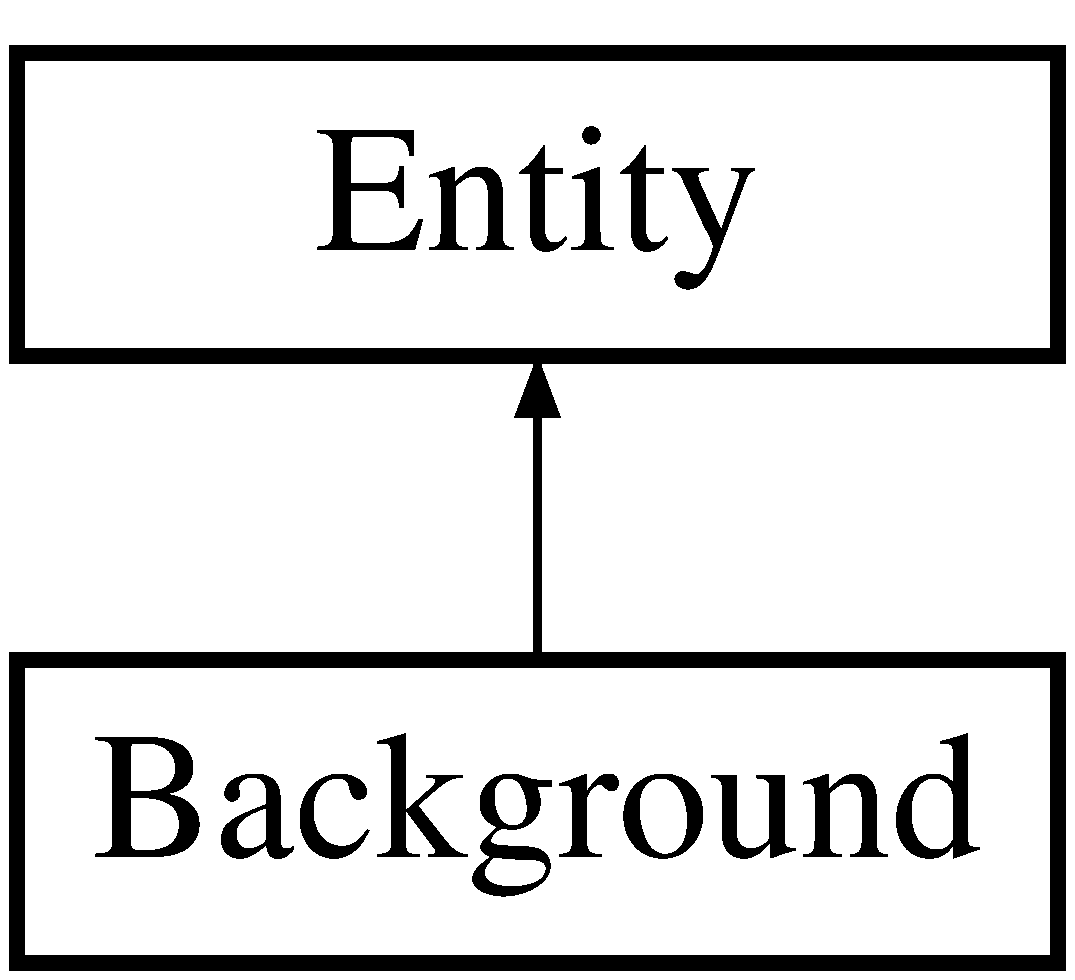
\includegraphics[height=2.000000cm]{class_background}
\end{center}
\end{figure}
\subsection*{Public Member Functions}
\begin{DoxyCompactItemize}
\item 
\mbox{\Hypertarget{class_background_a4e2392dc131ffee9384bbd65f49821cf}\label{class_background_a4e2392dc131ffee9384bbd65f49821cf}} 
{\bfseries Background} (float center\+Offset)
\item 
\mbox{\Hypertarget{class_background_af2356a6def94418c41c8ea8982186e68}\label{class_background_af2356a6def94418c41c8ea8982186e68}} 
Entity\+Types {\bfseries get\+Type} () const override
\end{DoxyCompactItemize}
\subsection*{Additional Inherited Members}


The documentation for this class was generated from the following file\+:\begin{DoxyCompactItemize}
\item 
Model/Background.\+h\end{DoxyCompactItemize}

\hypertarget{class_controller}{}\section{Controller Class Reference}
\label{class_controller}\index{Controller@{Controller}}
\subsection*{Public Member Functions}
\begin{DoxyCompactItemize}
\item 
\mbox{\Hypertarget{class_controller_afca093b5b1958be0bb60d3b9772f340f}\label{class_controller_afca093b5b1958be0bb60d3b9772f340f}} 
{\bfseries Controller} (std\+::shared\+\_\+ptr$<$ \hyperlink{class_model}{Model} $>$ model, std\+::shared\+\_\+ptr$<$ \hyperlink{class_view}{View} $>$ view)
\item 
void \hyperlink{class_controller_a692f0f5dc600cdcb79786a31cf283ce1}{run} ()
\end{DoxyCompactItemize}


\subsection{Member Function Documentation}
\mbox{\Hypertarget{class_controller_a692f0f5dc600cdcb79786a31cf283ce1}\label{class_controller_a692f0f5dc600cdcb79786a31cf283ce1}} 
\index{Controller@{Controller}!run@{run}}
\index{run@{run}!Controller@{Controller}}
\subsubsection{\texorpdfstring{run()}{run()}}
{\footnotesize\ttfamily void Controller\+::run (\begin{DoxyParamCaption}{ }\end{DoxyParamCaption})\hspace{0.3cm}{\ttfamily [inline]}}

C\+L\+O\+CK

poll event

get keyboard input 

The documentation for this class was generated from the following file\+:\begin{DoxyCompactItemize}
\item 
Controller/Controller.\+h\end{DoxyCompactItemize}

\hypertarget{struct_dimentions}{}\section{Dimensions Struct Reference}
\label{struct_dimentions}\index{Dimensions@{Dimensions}}
\subsection*{Public Member Functions}
\begin{DoxyCompactItemize}
\item 
\mbox{\Hypertarget{struct_dimentions_a09f92ee6239282f5d76c77d87f46f93e}\label{struct_dimentions_a09f92ee6239282f5d76c77d87f46f93e}} 
{\bfseries Dimensions} (float \+\_\+width, float \+\_\+height)
\end{DoxyCompactItemize}
\subsection*{Public Attributes}
\begin{DoxyCompactItemize}
\item 
\mbox{\Hypertarget{struct_dimentions_ab97c472cbe82f80e9a3a4f4c2ad9fe67}\label{struct_dimentions_ab97c472cbe82f80e9a3a4f4c2ad9fe67}} 
float {\bfseries width}
\item 
\mbox{\Hypertarget{struct_dimentions_a5481fb9860d7b293a20c720c027bae3a}\label{struct_dimentions_a5481fb9860d7b293a20c720c027bae3a}} 
float {\bfseries height}
\end{DoxyCompactItemize}


The documentation for this struct was generated from the following file\+:\begin{DoxyCompactItemize}
\item 
Helper\+Data\+Types.\+h\end{DoxyCompactItemize}

\hypertarget{class_enemy}{}\section{Enemy Class Reference}
\label{class_enemy}\index{Enemy@{Enemy}}
Inheritance diagram for Enemy\+:\begin{figure}[H]
\begin{center}
\leavevmode
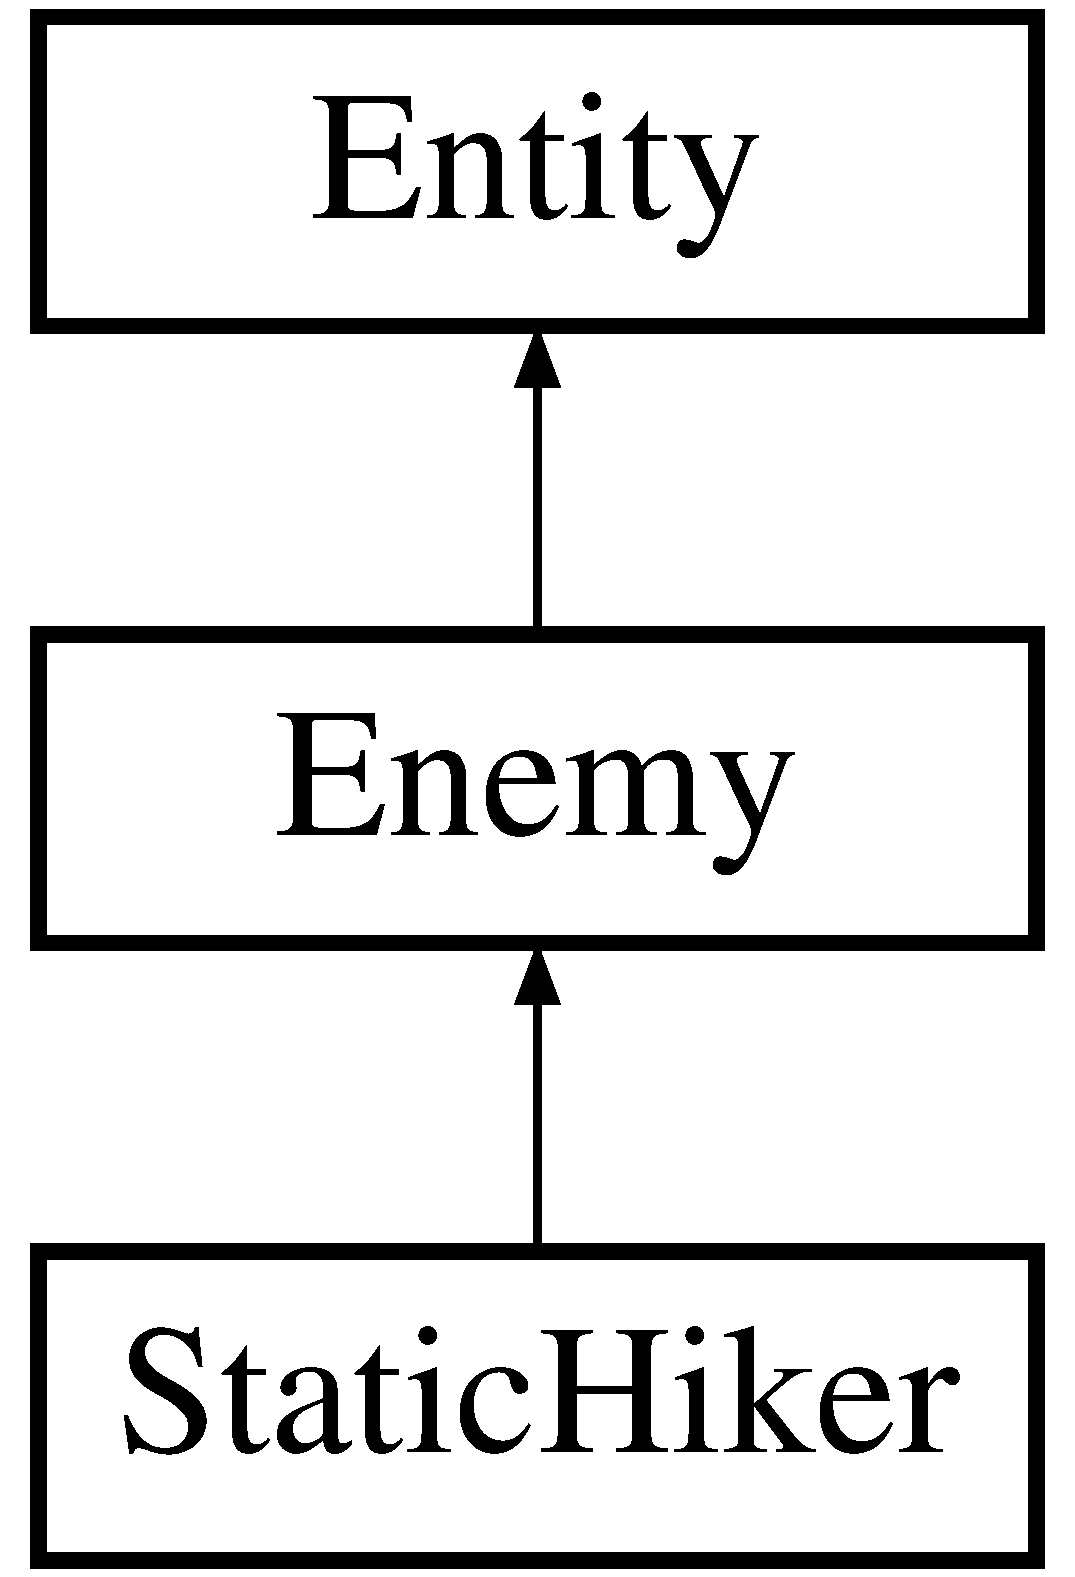
\includegraphics[height=3.000000cm]{class_enemy}
\end{center}
\end{figure}
\subsection*{Public Member Functions}
\begin{DoxyCompactItemize}
\item 
\mbox{\Hypertarget{class_enemy_a5ab16abc0999c739837711ccb1718b7f}\label{class_enemy_a5ab16abc0999c739837711ccb1718b7f}} 
bool {\bfseries is\+Collided} () const
\item 
\mbox{\Hypertarget{class_enemy_a74b115235415b4a4aef5899055730cdb}\label{class_enemy_a74b115235415b4a4aef5899055730cdb}} 
void {\bfseries set\+Collided} (bool collided)
\end{DoxyCompactItemize}
\subsection*{Protected Attributes}
\begin{DoxyCompactItemize}
\item 
\mbox{\Hypertarget{class_enemy_a9371fe2a8eb2188d6cbb5ab1d9349f73}\label{class_enemy_a9371fe2a8eb2188d6cbb5ab1d9349f73}} 
bool {\bfseries collided} \{false\}
\end{DoxyCompactItemize}


The documentation for this class was generated from the following files\+:\begin{DoxyCompactItemize}
\item 
Model/Enemy.\+h\item 
Model/Enemy.\+cpp\end{DoxyCompactItemize}

\hypertarget{class_entity}{}\section{Entity Class Reference}
\label{class_entity}\index{Entity@{Entity}}
Inheritance diagram for Entity\+:\begin{figure}[H]
\begin{center}
\leavevmode
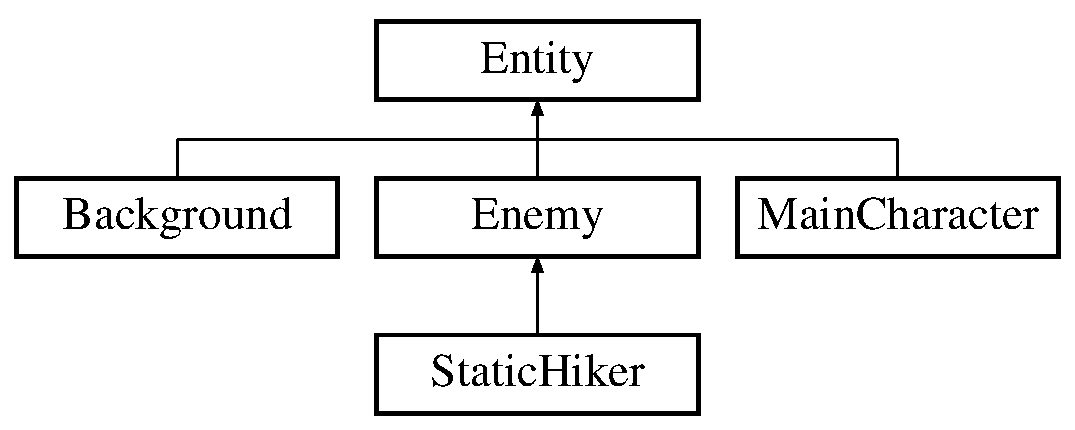
\includegraphics[height=3.000000cm]{class_entity}
\end{center}
\end{figure}
\subsection*{Public Member Functions}
\begin{DoxyCompactItemize}
\item 
\mbox{\Hypertarget{class_entity_a2ab2f30624fe669fd8fb72ab7a3e0318}\label{class_entity_a2ab2f30624fe669fd8fb72ab7a3e0318}} 
int {\bfseries get\+Skin} ()
\item 
\mbox{\Hypertarget{class_entity_a729e4d1d4a7f6f927f7fdf083c5dcc13}\label{class_entity_a729e4d1d4a7f6f927f7fdf083c5dcc13}} 
virtual Entity\+Types {\bfseries get\+Type} () const =0
\item 
\mbox{\Hypertarget{class_entity_a2234159416866c9c4657c9c481f0e632}\label{class_entity_a2234159416866c9c4657c9c481f0e632}} 
float {\bfseries get\+Movement\+Speed} () const
\item 
\mbox{\Hypertarget{class_entity_a5601a5a44bb9e13a001cbecb66154701}\label{class_entity_a5601a5a44bb9e13a001cbecb66154701}} 
std\+::shared\+\_\+ptr$<$ \hyperlink{struct_global_bounds}{Global\+Bounds} $>$ {\bfseries get\+Global\+Bounds} () const
\item 
\mbox{\Hypertarget{class_entity_a93306ecdce9446da37560f5f2b5307c0}\label{class_entity_a93306ecdce9446da37560f5f2b5307c0}} 
void {\bfseries set\+Position} (float x, float y)
\item 
\mbox{\Hypertarget{class_entity_a474692558c0fcb4f3d0b931022b847d8}\label{class_entity_a474692558c0fcb4f3d0b931022b847d8}} 
void {\bfseries move} (float offsetX, float offsetY)
\item 
{\footnotesize template$<$typename type $>$ }\\bool \hyperlink{class_entity_a6dcfeadddb85cce9f5352b6553ab404b}{intersects} (const std\+::shared\+\_\+ptr$<$ \hyperlink{struct_global_bounds}{Global\+Bounds} $>$ \&next\+Position) const
\end{DoxyCompactItemize}
\subsection*{Protected Attributes}
\begin{DoxyCompactItemize}
\item 
\mbox{\Hypertarget{class_entity_a153419f3400cd95918a437083b371eb3}\label{class_entity_a153419f3400cd95918a437083b371eb3}} 
int {\bfseries skin} \{-\/1\}
\item 
\mbox{\Hypertarget{class_entity_ae604454cbac259c1229a0a142d4c02d0}\label{class_entity_ae604454cbac259c1229a0a142d4c02d0}} 
std\+::shared\+\_\+ptr$<$ \hyperlink{struct_global_bounds}{Global\+Bounds} $>$ {\bfseries global\+Bounds}
\item 
\mbox{\Hypertarget{class_entity_ac28cd407994c232f1b71c886bb9aa584}\label{class_entity_ac28cd407994c232f1b71c886bb9aa584}} 
float {\bfseries movement\+Speed}
\end{DoxyCompactItemize}


\subsection{Member Function Documentation}
\mbox{\Hypertarget{class_entity_a6dcfeadddb85cce9f5352b6553ab404b}\label{class_entity_a6dcfeadddb85cce9f5352b6553ab404b}} 
\index{Entity@{Entity}!intersects@{intersects}}
\index{intersects@{intersects}!Entity@{Entity}}
\subsubsection{\texorpdfstring{intersects()}{intersects()}}
{\footnotesize\ttfamily template$<$typename type $>$ \\
bool Entity\+::intersects (\begin{DoxyParamCaption}\item[{const std\+::shared\+\_\+ptr$<$ \hyperlink{struct_global_bounds}{Global\+Bounds} $>$ \&}]{next\+Position }\end{DoxyParamCaption}) const\hspace{0.3cm}{\ttfamily [inline]}}

Keep in mind that we are working with rectangle objects 
\begin{DoxyParams}{Parameters}
{\em next\+Position} & \\
\hline
\end{DoxyParams}
\begin{DoxyReturn}{Returns}

\end{DoxyReturn}


The documentation for this class was generated from the following files\+:\begin{DoxyCompactItemize}
\item 
Model/Entity.\+h\item 
Model/Entity.\+cpp\end{DoxyCompactItemize}

\hypertarget{class_entity_maker}{}\section{Entity\+Maker Class Reference}
\label{class_entity_maker}\index{Entity\+Maker@{Entity\+Maker}}
\subsection*{Public Member Functions}
\begin{DoxyCompactItemize}
\item 
\mbox{\Hypertarget{class_entity_maker_a6df64267ba7e9ae80a5c6ecf3805029f}\label{class_entity_maker_a6df64267ba7e9ae80a5c6ecf3805029f}} 
std\+::shared\+\_\+ptr$<$ \hyperlink{class_main_character}{Main\+Character} $>$ {\bfseries generate\+Main\+Character} (int lanes)
\item 
\mbox{\Hypertarget{class_entity_maker_a5253324877ee4cb0eec7868f6fb8c36c}\label{class_entity_maker_a5253324877ee4cb0eec7868f6fb8c36c}} 
std\+::vector$<$ std\+::shared\+\_\+ptr$<$ \hyperlink{class_enemy}{Enemy} $>$ $>$ {\bfseries generate\+Enemies} ()
\item 
\mbox{\Hypertarget{class_entity_maker_a74af0a50deaa3dce647359d53f01f7fd}\label{class_entity_maker_a74af0a50deaa3dce647359d53f01f7fd}} 
std\+::vector$<$ std\+::shared\+\_\+ptr$<$ \hyperlink{class_background}{Background} $>$ $>$ {\bfseries generate\+Background} ()
\end{DoxyCompactItemize}


The documentation for this class was generated from the following file\+:\begin{DoxyCompactItemize}
\item 
Model/Entity\+Maker.\+h\end{DoxyCompactItemize}

\hypertarget{struct_global_bounds}{}\section{Global\+Bounds Struct Reference}
\label{struct_global_bounds}\index{Global\+Bounds@{Global\+Bounds}}
\subsection*{Public Member Functions}
\begin{DoxyCompactItemize}
\item 
\mbox{\Hypertarget{struct_global_bounds_a38d87fc7f3c34bff62bd744ac9fc3724}\label{struct_global_bounds_a38d87fc7f3c34bff62bd744ac9fc3724}} 
{\bfseries Global\+Bounds} (\hyperlink{struct_position}{Position} \&pos, \hyperlink{struct_dimentions}{Dimentions} \&dim)
\end{DoxyCompactItemize}
\subsection*{Public Attributes}
\begin{DoxyCompactItemize}
\item 
\mbox{\Hypertarget{struct_global_bounds_a6224bede2eff12cec85b6999b7faedc3}\label{struct_global_bounds_a6224bede2eff12cec85b6999b7faedc3}} 
\hyperlink{struct_position}{Position} {\bfseries position}
\item 
\mbox{\Hypertarget{struct_global_bounds_a1fb273eb005424a1d6ff34d3808c7081}\label{struct_global_bounds_a1fb273eb005424a1d6ff34d3808c7081}} 
\hyperlink{struct_dimentions}{Dimentions} {\bfseries dimentions}
\end{DoxyCompactItemize}


The documentation for this struct was generated from the following file\+:\begin{DoxyCompactItemize}
\item 
Helper\+Data\+Types.\+h\end{DoxyCompactItemize}

\hypertarget{class_main_character}{}\section{Main\+Character Class Reference}
\label{class_main_character}\index{Main\+Character@{Main\+Character}}
Inheritance diagram for Main\+Character\+:\begin{figure}[H]
\begin{center}
\leavevmode
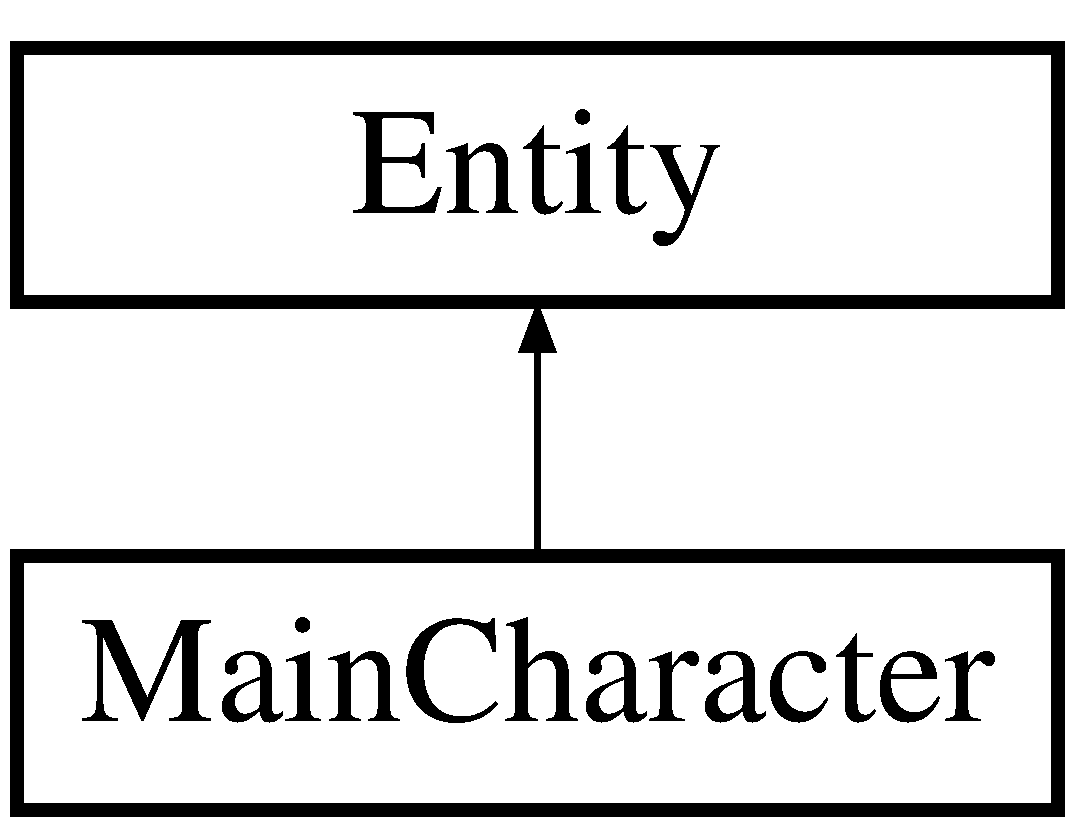
\includegraphics[height=2.000000cm]{class_main_character}
\end{center}
\end{figure}
\subsection*{Public Member Functions}
\begin{DoxyCompactItemize}
\item 
\hyperlink{class_main_character_aacd15121a3f8cab760aec751e348e17d}{Main\+Character} (int lanes)
\item 
\mbox{\Hypertarget{class_main_character_ac3acc3f570b8f8024ec760ab4e738cde}\label{class_main_character_ac3acc3f570b8f8024ec760ab4e738cde}} 
Entity\+Types {\bfseries get\+Type} () const override
\end{DoxyCompactItemize}
\subsection*{Additional Inherited Members}


\subsection{Constructor \& Destructor Documentation}
\mbox{\Hypertarget{class_main_character_aacd15121a3f8cab760aec751e348e17d}\label{class_main_character_aacd15121a3f8cab760aec751e348e17d}} 
\index{Main\+Character@{Main\+Character}!Main\+Character@{Main\+Character}}
\index{Main\+Character@{Main\+Character}!Main\+Character@{Main\+Character}}
\subsubsection{\texorpdfstring{Main\+Character()}{MainCharacter()}}
{\footnotesize\ttfamily Main\+Character\+::\+Main\+Character (\begin{DoxyParamCaption}\item[{int}]{lanes }\end{DoxyParamCaption})}

in a (-\/4,4) (-\/3,3) coordinate system. Our character needs to be placed at the lowest-\/middle part of the screen screen\+: 6 

 \tabulinesep=1mm
\begin{longtabu} spread 0pt [c]{*{1}{|X[-1]}|}
\hline
\rowcolor{\tableheadbgcolor}\textbf{ }\\\cline{1-1}
\endfirsthead
\hline
\endfoot
\hline
\rowcolor{\tableheadbgcolor}\textbf{ }\\\cline{1-1}
\endhead
\\\cline{1-1}
\end{longtabu}
8 $\vert$ $\vert$ \tabulinesep=1mm
\begin{longtabu} spread 0pt [c]{*{1}{|X[-1]}|}
\hline
\rowcolor{\tableheadbgcolor}\textbf{ }\\\cline{1-1}
\endfirsthead
\hline
\endfoot
\hline
\rowcolor{\tableheadbgcolor}\textbf{ }\\\cline{1-1}
\endhead
\+\_\+\+\_\+\+\_\+\+\_\+\+\_\+char\+\_\+\+\_\+\+\_\+\+\_\+\+\_\+ \\\cline{1-1}
\end{longtabu}
todo\+: 8 divided by lanes doesnt really make sense; 

The documentation for this class was generated from the following files\+:\begin{DoxyCompactItemize}
\item 
Model/Main\+Character.\+h\item 
Model/Main\+Character.\+cpp\end{DoxyCompactItemize}

\hypertarget{class_model}{}\section{Model Class Reference}
\label{class_model}\index{Model@{Model}}
\subsection*{Public Member Functions}
\begin{DoxyCompactItemize}
\item 
\mbox{\Hypertarget{class_model_a8352e72694201310bb9547964f33805e}\label{class_model_a8352e72694201310bb9547964f33805e}} 
const \hyperlink{struct_move}{Move} \& {\bfseries get\+Player\+Move} () const
\item 
\mbox{\Hypertarget{class_model_a0244b243926e1a87c665f3ad5e93f969}\label{class_model_a0244b243926e1a87c665f3ad5e93f969}} 
void {\bfseries set\+Player\+MoveX} (const float \&moveX)
\item 
\mbox{\Hypertarget{class_model_aaf51aa15e5207002ab11bab7bc5ddf53}\label{class_model_aaf51aa15e5207002ab11bab7bc5ddf53}} 
void {\bfseries set\+Player\+MoveY} (const float \&moveY)
\item 
\mbox{\Hypertarget{class_model_ae1dba27e8f978f6a0a88f19eaa7d4c35}\label{class_model_ae1dba27e8f978f6a0a88f19eaa7d4c35}} 
const \hyperlink{struct_move}{Move} \& {\bfseries get\+Background\+Move} () const
\item 
\mbox{\Hypertarget{class_model_ac28ab3c0e3b6d7c18b6a73e7b9751d37}\label{class_model_ac28ab3c0e3b6d7c18b6a73e7b9751d37}} 
void {\bfseries set\+Background\+MoveY} (const float \&moveY)
\item 
\mbox{\Hypertarget{class_model_acbf5b4b8802d6b98edd508abfc447d01}\label{class_model_acbf5b4b8802d6b98edd508abfc447d01}} 
{\bfseries Model} (float frame\+Limit)
\item 
\mbox{\Hypertarget{class_model_aa4c3ab6b5c637225bd1136ca0b703344}\label{class_model_aa4c3ab6b5c637225bd1136ca0b703344}} 
float {\bfseries get\+Fps} () const
\item 
\mbox{\Hypertarget{class_model_a4c501d09ee4fa6bcb9b93a20781e2e70}\label{class_model_a4c501d09ee4fa6bcb9b93a20781e2e70}} 
std\+::shared\+\_\+ptr$<$ \hyperlink{class_main_character}{Main\+Character} $>$ {\bfseries get\+Main\+Character} () const
\item 
\mbox{\Hypertarget{class_model_aecbb3a282ee591c997375c8bc77ce174}\label{class_model_aecbb3a282ee591c997375c8bc77ce174}} 
std\+::vector$<$ std\+::shared\+\_\+ptr$<$ \hyperlink{class_background}{Background} $>$ $>$ {\bfseries get\+Backgrounds} () const
\item 
\mbox{\Hypertarget{class_model_ad2adcd81ad4cdd73b3db10a4e807caf4}\label{class_model_ad2adcd81ad4cdd73b3db10a4e807caf4}} 
std\+::vector$<$ std\+::shared\+\_\+ptr$<$ \hyperlink{class_enemy}{Enemy} $>$ $>$ {\bfseries get\+Enemies} ()
\item 
\mbox{\Hypertarget{class_model_ad95392ecd55444f93ca2f471f2c97b09}\label{class_model_ad95392ecd55444f93ca2f471f2c97b09}} 
std\+::shared\+\_\+ptr$<$ \hyperlink{class_main_character}{Main\+Character} $>$ {\bfseries generate\+MC} ()
\item 
\mbox{\Hypertarget{class_model_ab50b67ca385d1ab402ded5ecec7b96cc}\label{class_model_ab50b67ca385d1ab402ded5ecec7b96cc}} 
std\+::vector$<$ std\+::shared\+\_\+ptr$<$ \hyperlink{class_background}{Background} $>$ $>$ {\bfseries generate\+Background} ()
\item 
std\+::vector$<$ std\+::shared\+\_\+ptr$<$ \hyperlink{class_enemy}{Enemy} $>$ $>$ \hyperlink{class_model_a37263d57b165877f36157a9538c0b96b}{generate\+Enemies} ()
\item 
\mbox{\Hypertarget{class_model_af6ca3e8ebb3b6ac3a0d0d413e33e8693}\label{class_model_af6ca3e8ebb3b6ac3a0d0d413e33e8693}} 
void {\bfseries reset\+Moves} ()
\item 
\mbox{\Hypertarget{class_model_ae330be8cd03370cc346432543b361c35}\label{class_model_ae330be8cd03370cc346432543b361c35}} 
void {\bfseries move\+MC} ()
\item 
\mbox{\Hypertarget{class_model_ad7a90c028065c2baa83ee34904c3ded7}\label{class_model_ad7a90c028065c2baa83ee34904c3ded7}} 
void {\bfseries move\+Background} ()
\item 
\mbox{\Hypertarget{class_model_aa8caf28eae1565d64633db18b0f4f5a6}\label{class_model_aa8caf28eae1565d64633db18b0f4f5a6}} 
void {\bfseries move\+Enemies} ()
\item 
void \hyperlink{class_model_a342131d5e48ed3ab8d59f9b19c7f759a}{screen\+Collision\+Control} ()
\item 
void \hyperlink{class_model_a66849d75ce129d37a71eeec94e4b6d3d}{collision\+Control} ()
\end{DoxyCompactItemize}


\subsection{Member Function Documentation}
\mbox{\Hypertarget{class_model_a66849d75ce129d37a71eeec94e4b6d3d}\label{class_model_a66849d75ce129d37a71eeec94e4b6d3d}} 
\index{Model@{Model}!collision\+Control@{collision\+Control}}
\index{collision\+Control@{collision\+Control}!Model@{Model}}
\subsubsection{\texorpdfstring{collision\+Control()}{collisionControl()}}
{\footnotesize\ttfamily void Model\+::collision\+Control (\begin{DoxyParamCaption}{ }\end{DoxyParamCaption})\hspace{0.3cm}{\ttfamily [inline]}}

possible solution1\+: set player\+Move x and y to 0 possible solution2\+: first construct left and right collision, bottom-\/top is simillar but inverted \mbox{\Hypertarget{class_model_a37263d57b165877f36157a9538c0b96b}\label{class_model_a37263d57b165877f36157a9538c0b96b}} 
\index{Model@{Model}!generate\+Enemies@{generate\+Enemies}}
\index{generate\+Enemies@{generate\+Enemies}!Model@{Model}}
\subsubsection{\texorpdfstring{generate\+Enemies()}{generateEnemies()}}
{\footnotesize\ttfamily std\+::vector$<$std\+::shared\+\_\+ptr$<$\hyperlink{class_enemy}{Enemy}$>$ $>$ Model\+::generate\+Enemies (\begin{DoxyParamCaption}{ }\end{DoxyParamCaption})\hspace{0.3cm}{\ttfamily [inline]}}

Generates enemies of random types spawning them at the top part of the screen \begin{DoxyReturn}{Returns}
A vector of generated enemies 
\end{DoxyReturn}
\mbox{\Hypertarget{class_model_a342131d5e48ed3ab8d59f9b19c7f759a}\label{class_model_a342131d5e48ed3ab8d59f9b19c7f759a}} 
\index{Model@{Model}!screen\+Collision\+Control@{screen\+Collision\+Control}}
\index{screen\+Collision\+Control@{screen\+Collision\+Control}!Model@{Model}}
\subsubsection{\texorpdfstring{screen\+Collision\+Control()}{screenCollisionControl()}}
{\footnotesize\ttfamily void Model\+::screen\+Collision\+Control (\begin{DoxyParamCaption}{ }\end{DoxyParamCaption})\hspace{0.3cm}{\ttfamily [inline]}}

Window collision control left collision

right collision 

The documentation for this class was generated from the following files\+:\begin{DoxyCompactItemize}
\item 
Model/Model.\+h\item 
Model/Model.\+cpp\end{DoxyCompactItemize}

\hypertarget{struct_move}{}\section{Move Struct Reference}
\label{struct_move}\index{Move@{Move}}
\subsection*{Public Attributes}
\begin{DoxyCompactItemize}
\item 
\mbox{\Hypertarget{struct_move_a15a4723eb1501a58104bbffaf71ae297}\label{struct_move_a15a4723eb1501a58104bbffaf71ae297}} 
float {\bfseries x}
\item 
\mbox{\Hypertarget{struct_move_ad9a7db3b23380854c8859c619e0d64b8}\label{struct_move_ad9a7db3b23380854c8859c619e0d64b8}} 
float {\bfseries y}
\end{DoxyCompactItemize}


The documentation for this struct was generated from the following file\+:\begin{DoxyCompactItemize}
\item 
Helper\+Data\+Types.\+h\end{DoxyCompactItemize}

\hypertarget{struct_position}{}\section{Position Struct Reference}
\label{struct_position}\index{Position@{Position}}


{\ttfamily \#include $<$Helper\+Data\+Types.\+h$>$}

\subsection*{Public Member Functions}
\begin{DoxyCompactItemize}
\item 
\mbox{\Hypertarget{struct_position_a2846e4a9e095a0f98f5be27936af63db}\label{struct_position_a2846e4a9e095a0f98f5be27936af63db}} 
{\bfseries Position} (float x\+Cor, float y\+Cor)
\end{DoxyCompactItemize}
\subsection*{Public Attributes}
\begin{DoxyCompactItemize}
\item 
\mbox{\Hypertarget{struct_position_af684446cbf0f6d53386686283da6dcc6}\label{struct_position_af684446cbf0f6d53386686283da6dcc6}} 
float {\bfseries x}
\item 
\mbox{\Hypertarget{struct_position_a54a6182b5f7539295b32255808897d3f}\label{struct_position_a54a6182b5f7539295b32255808897d3f}} 
float {\bfseries y}
\end{DoxyCompactItemize}


\subsection{Detailed Description}
structure used to specify the coordinates of a given entity 

The documentation for this struct was generated from the following file\+:\begin{DoxyCompactItemize}
\item 
Helper\+Data\+Types.\+h\end{DoxyCompactItemize}

\hypertarget{class_random}{}\section{Random Class Reference}
\label{class_random}\index{Random@{Random}}
\subsection*{Public Member Functions}
\begin{DoxyCompactItemize}
\item 
int \hyperlink{class_random_a35a3289bf89b45e55c3cb69bf36453c2}{int\+In\+Interval} (const int \&left, const int \&right) const
\item 
float \hyperlink{class_random_ab74f1a7b95a41426f87698f400b382e8}{float\+In\+Interval} (const float \&left, const float \&right) const
\end{DoxyCompactItemize}
\subsection*{Static Public Member Functions}
\begin{DoxyCompactItemize}
\item 
\mbox{\Hypertarget{class_random_af3f69a0efaceb95bec54043d4becda09}\label{class_random_af3f69a0efaceb95bec54043d4becda09}} 
static std\+::shared\+\_\+ptr$<$ \hyperlink{class_random}{Random} $>$ {\bfseries get\+Instance} ()
\end{DoxyCompactItemize}


\subsection{Member Function Documentation}
\mbox{\Hypertarget{class_random_ab74f1a7b95a41426f87698f400b382e8}\label{class_random_ab74f1a7b95a41426f87698f400b382e8}} 
\index{Random@{Random}!float\+In\+Interval@{float\+In\+Interval}}
\index{float\+In\+Interval@{float\+In\+Interval}!Random@{Random}}
\subsubsection{\texorpdfstring{float\+In\+Interval()}{floatInInterval()}}
{\footnotesize\ttfamily float Random\+::float\+In\+Interval (\begin{DoxyParamCaption}\item[{const float \&}]{left,  }\item[{const float \&}]{right }\end{DoxyParamCaption}) const\hspace{0.3cm}{\ttfamily [inline]}}


\begin{DoxyParams}{Parameters}
{\em left} & \+: The leftmost limit within our range \\
\hline
{\em right} & \+: The rightmost limit within our range \\
\hline
\end{DoxyParams}
\begin{DoxyReturn}{Returns}
A random float generated from a uniform distribution 
\end{DoxyReturn}
\mbox{\Hypertarget{class_random_a35a3289bf89b45e55c3cb69bf36453c2}\label{class_random_a35a3289bf89b45e55c3cb69bf36453c2}} 
\index{Random@{Random}!int\+In\+Interval@{int\+In\+Interval}}
\index{int\+In\+Interval@{int\+In\+Interval}!Random@{Random}}
\subsubsection{\texorpdfstring{int\+In\+Interval()}{intInInterval()}}
{\footnotesize\ttfamily int Random\+::int\+In\+Interval (\begin{DoxyParamCaption}\item[{const int \&}]{left,  }\item[{const int \&}]{right }\end{DoxyParamCaption}) const\hspace{0.3cm}{\ttfamily [inline]}}


\begin{DoxyParams}{Parameters}
{\em left} & \+: The leftmost limit within our range \\
\hline
{\em right} & \+: The rightmost limit within our range \\
\hline
\end{DoxyParams}
\begin{DoxyReturn}{Returns}
A random number generated from a uniform distribution 
\end{DoxyReturn}


The documentation for this class was generated from the following files\+:\begin{DoxyCompactItemize}
\item 
Singletons/Random.\+h\item 
Singletons/Random.\+cpp\end{DoxyCompactItemize}

\hypertarget{class_static_hiker}{}\section{Static\+Hiker Class Reference}
\label{class_static_hiker}\index{Static\+Hiker@{Static\+Hiker}}
Inheritance diagram for Static\+Hiker\+:\begin{figure}[H]
\begin{center}
\leavevmode
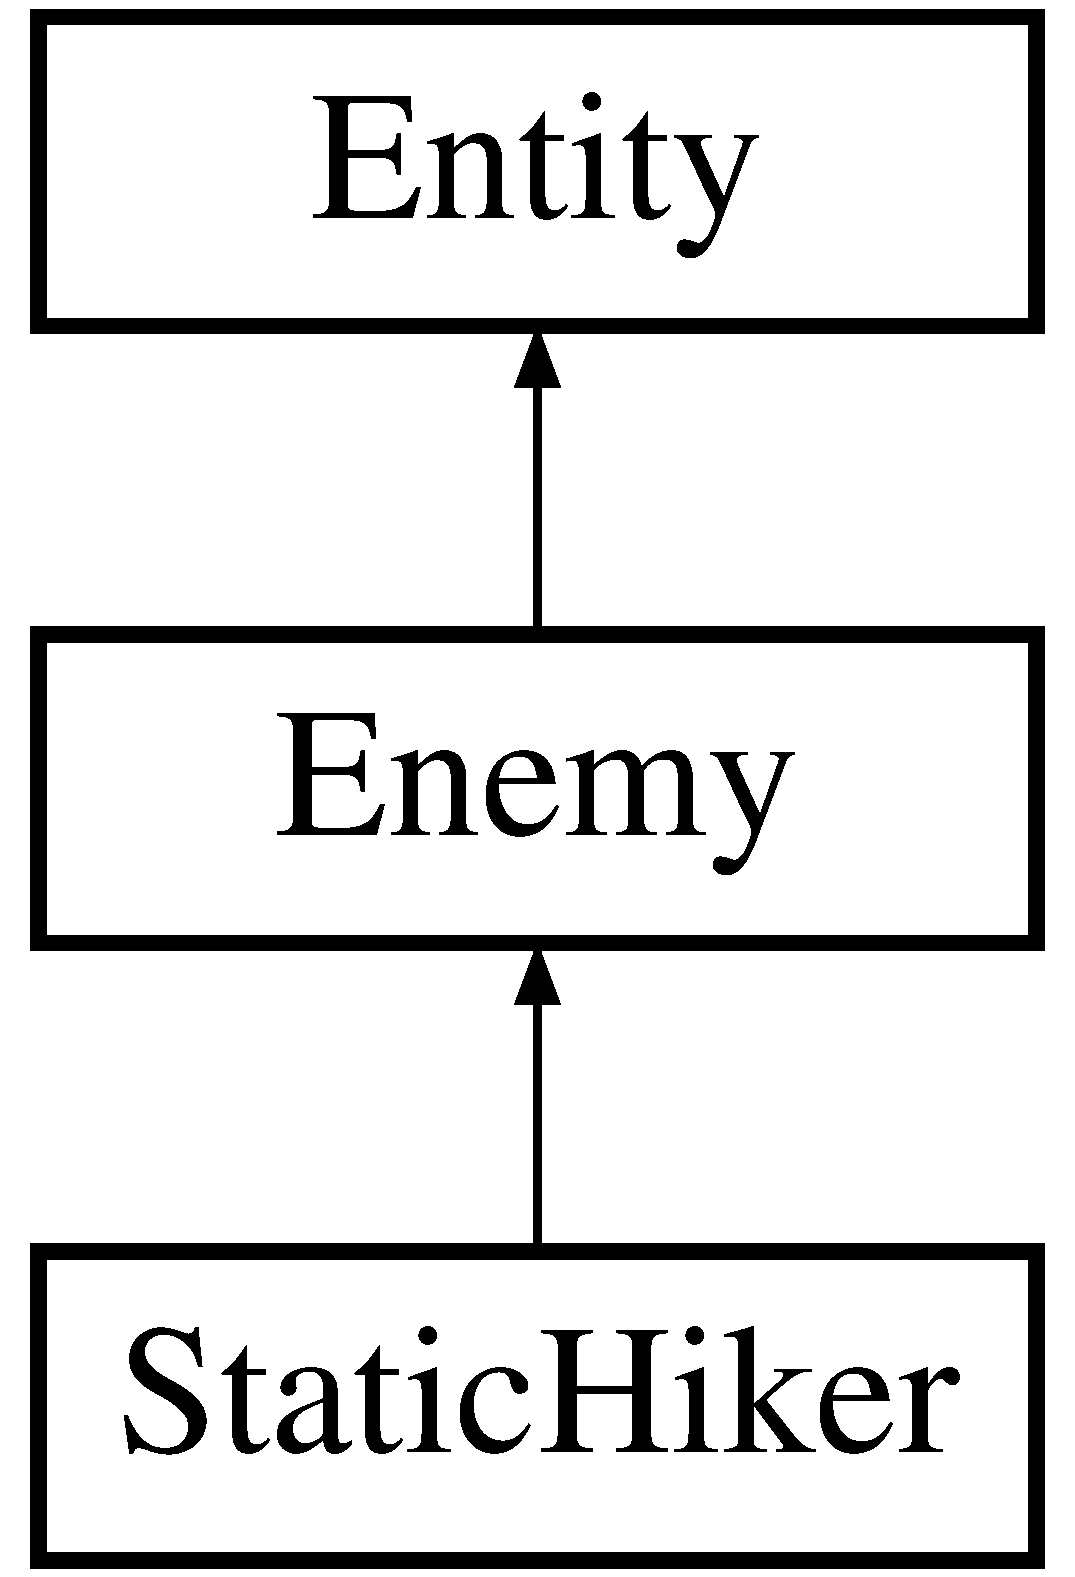
\includegraphics[height=3.000000cm]{class_static_hiker}
\end{center}
\end{figure}
\subsection*{Public Member Functions}
\begin{DoxyCompactItemize}
\item 
\hyperlink{class_static_hiker_abdeca694baaf9fe7e69d968d49a8e75f}{Static\+Hiker} (const int \&horizontal\+Offset)
\item 
\mbox{\Hypertarget{class_static_hiker_ac24096f5b7efbd98cf17adc968b6ffa6}\label{class_static_hiker_ac24096f5b7efbd98cf17adc968b6ffa6}} 
Entity\+Types {\bfseries get\+Type} () const override
\end{DoxyCompactItemize}
\subsection*{Additional Inherited Members}


\subsection{Constructor \& Destructor Documentation}
\mbox{\Hypertarget{class_static_hiker_abdeca694baaf9fe7e69d968d49a8e75f}\label{class_static_hiker_abdeca694baaf9fe7e69d968d49a8e75f}} 
\index{Static\+Hiker@{Static\+Hiker}!Static\+Hiker@{Static\+Hiker}}
\index{Static\+Hiker@{Static\+Hiker}!Static\+Hiker@{Static\+Hiker}}
\subsubsection{\texorpdfstring{Static\+Hiker()}{StaticHiker()}}
{\footnotesize\ttfamily Static\+Hiker\+::\+Static\+Hiker (\begin{DoxyParamCaption}\item[{const int \&}]{horizontal\+Offset }\end{DoxyParamCaption})\hspace{0.3cm}{\ttfamily [explicit]}}

Initializes a static hiker given a horizontal offset 
\begin{DoxyParams}{Parameters}
{\em horizontal\+Offset} & \\
\hline
\end{DoxyParams}
todo\+: 8 divided by lanes doesnt really make sense; 

The documentation for this class was generated from the following files\+:\begin{DoxyCompactItemize}
\item 
Model/Static\+Hiker.\+h\item 
Model/Static\+Hiker.\+cpp\end{DoxyCompactItemize}

\hypertarget{classsingleton_1_1_transformation}{}\section{singleton\+:\+:Transformation Class Reference}
\label{classsingleton_1_1_transformation}\index{singleton\+::\+Transformation@{singleton\+::\+Transformation}}
\subsection*{Public Member Functions}
\begin{DoxyCompactItemize}
\item 
\mbox{\Hypertarget{classsingleton_1_1_transformation_a45a811840e91388f25054019c28a27cd}\label{classsingleton_1_1_transformation_a45a811840e91388f25054019c28a27cd}} 
const \hyperlink{struct_dimentions}{Dimentions} \& {\bfseries get\+Screen\+Dimentions} ()
\item 
std\+::tuple$<$ float, float $>$ \hyperlink{classsingleton_1_1_transformation_a4db8bb77746a79641a057c19b30785c6}{model\+To\+View} (const std\+::shared\+\_\+ptr$<$ \hyperlink{struct_global_bounds}{Global\+Bounds} $>$ \&global\+Bounds) const
\item 
\mbox{\Hypertarget{classsingleton_1_1_transformation_afc296e4278c48d0ab5345192e189669e}\label{classsingleton_1_1_transformation_afc296e4278c48d0ab5345192e189669e}} 
std\+::tuple$<$ float, float $>$ {\bfseries view\+To\+Model} (float x, float y) const
\end{DoxyCompactItemize}
\subsection*{Static Public Member Functions}
\begin{DoxyCompactItemize}
\item 
\mbox{\Hypertarget{classsingleton_1_1_transformation_ab4f0dbbfe1889d5c9f1b70131ba640d5}\label{classsingleton_1_1_transformation_ab4f0dbbfe1889d5c9f1b70131ba640d5}} 
static std\+::shared\+\_\+ptr$<$ \hyperlink{classsingleton_1_1_transformation}{Transformation} $>$ {\bfseries get\+Instance} ()
\item 
\mbox{\Hypertarget{classsingleton_1_1_transformation_acef1b7fefa4473eaa785eb42b8ae6066}\label{classsingleton_1_1_transformation_acef1b7fefa4473eaa785eb42b8ae6066}} 
static std\+::shared\+\_\+ptr$<$ \hyperlink{classsingleton_1_1_transformation}{Transformation} $>$ {\bfseries init} (\hyperlink{struct_dimentions}{Dimentions} dimentions)
\end{DoxyCompactItemize}


\subsection{Member Function Documentation}
\mbox{\Hypertarget{classsingleton_1_1_transformation_a4db8bb77746a79641a057c19b30785c6}\label{classsingleton_1_1_transformation_a4db8bb77746a79641a057c19b30785c6}} 
\index{singleton\+::\+Transformation@{singleton\+::\+Transformation}!model\+To\+View@{model\+To\+View}}
\index{model\+To\+View@{model\+To\+View}!singleton\+::\+Transformation@{singleton\+::\+Transformation}}
\subsubsection{\texorpdfstring{model\+To\+View()}{modelToView()}}
{\footnotesize\ttfamily std\+::tuple$<$float, float$>$ singleton\+::\+Transformation\+::model\+To\+View (\begin{DoxyParamCaption}\item[{const std\+::shared\+\_\+ptr$<$ \hyperlink{struct_global_bounds}{Global\+Bounds} $>$ \&}]{global\+Bounds }\end{DoxyParamCaption}) const\hspace{0.3cm}{\ttfamily [inline]}}

converts the model\textquotesingle{}s (0,6) (0,8) coordinate system into the \hyperlink{class_view}{View}\textquotesingle{}s (0, screen\+Width) (0, screen\+Height) coordinate system 
\begin{DoxyParams}{Parameters}
{\em coords} & \\
\hline
{\em screen\+Width} & \\
\hline
{\em screen\+Height} & \\
\hline
\end{DoxyParams}
\begin{DoxyReturn}{Returns}

\end{DoxyReturn}


The documentation for this class was generated from the following files\+:\begin{DoxyCompactItemize}
\item 
Singletons/Transformation.\+h\item 
Singletons/Transformation.\+cpp\end{DoxyCompactItemize}

\hypertarget{class_turbo_hiker}{}\section{Turbo\+Hiker Class Reference}
\label{class_turbo_hiker}\index{Turbo\+Hiker@{Turbo\+Hiker}}
\subsection*{Public Member Functions}
\begin{DoxyCompactItemize}
\item 
\mbox{\Hypertarget{class_turbo_hiker_afcd90c00a28da42a494c850ca1bcc57f}\label{class_turbo_hiker_afcd90c00a28da42a494c850ca1bcc57f}} 
{\bfseries Turbo\+Hiker} (float fps)
\item 
\mbox{\Hypertarget{class_turbo_hiker_aba075b3c3bcec452730826893ba60c87}\label{class_turbo_hiker_aba075b3c3bcec452730826893ba60c87}} 
void {\bfseries run} ()
\end{DoxyCompactItemize}


The documentation for this class was generated from the following file\+:\begin{DoxyCompactItemize}
\item 
Turbo\+Hiker.\+h\end{DoxyCompactItemize}

\hypertarget{class_view}{}\section{View Class Reference}
\label{class_view}\index{View@{View}}
\subsection*{Public Member Functions}
\begin{DoxyCompactItemize}
\item 
\mbox{\Hypertarget{class_view_aa8b502dd59a99ba0ec5c961b099cd443}\label{class_view_aa8b502dd59a99ba0ec5c961b099cd443}} 
const sf\+::\+Render\+Window \& {\bfseries get\+Window} () const
\item 
\hyperlink{class_view_a11dfb2fbc3e20eb48c96b8e8a20687cb}{View} (const float fps)
\item 
\mbox{\Hypertarget{class_view_a810ac2903e9bdbdcd3d92b677fc0e7e0}\label{class_view_a810ac2903e9bdbdcd3d92b677fc0e7e0}} 
void {\bfseries initialize\+Window} (const float fps)
\item 
\mbox{\Hypertarget{class_view_af3b02b172b87fc315a98ce00f86074d4}\label{class_view_af3b02b172b87fc315a98ce00f86074d4}} 
void {\bfseries load\+Textures} ()
\item 
\mbox{\Hypertarget{class_view_ab94417a6b73c205cece8432b7ab4458a}\label{class_view_ab94417a6b73c205cece8432b7ab4458a}} 
void {\bfseries assign\+B\+Gand\+M\+C\+Textures} ()
\item 
\mbox{\Hypertarget{class_view_a0a285a78bd5d06cbef88dcbd0ad9a022}\label{class_view_a0a285a78bd5d06cbef88dcbd0ad9a022}} 
Input {\bfseries poll\+Event} ()
\item 
\mbox{\Hypertarget{class_view_ae8d33c17a56173d3ef8f6ab47a1568d7}\label{class_view_ae8d33c17a56173d3ef8f6ab47a1568d7}} 
Input {\bfseries get\+Keyboard\+Input} ()
\item 
\mbox{\Hypertarget{class_view_a30af1accdfddafd1318d301092934d67}\label{class_view_a30af1accdfddafd1318d301092934d67}} 
void {\bfseries draw2} (const std\+::shared\+\_\+ptr$<$ \hyperlink{class_main_character}{Main\+Character} $>$ \&mc, const std\+::vector$<$ std\+::shared\+\_\+ptr$<$ \hyperlink{class_background}{Background} $>$$>$ \&backgrounds, const std\+::vector$<$ std\+::shared\+\_\+ptr$<$ \hyperlink{class_enemy}{Enemy} $>$$>$ \&enemies)
\item 
void \hyperlink{class_view_ad26b8f3c6e07b3a8292ad508c5d081b5}{draw} ()
\end{DoxyCompactItemize}


\subsection{Constructor \& Destructor Documentation}
\mbox{\Hypertarget{class_view_a11dfb2fbc3e20eb48c96b8e8a20687cb}\label{class_view_a11dfb2fbc3e20eb48c96b8e8a20687cb}} 
\index{View@{View}!View@{View}}
\index{View@{View}!View@{View}}
\subsubsection{\texorpdfstring{View()}{View()}}
{\footnotesize\ttfamily View\+::\+View (\begin{DoxyParamCaption}\item[{const float}]{fps }\end{DoxyParamCaption})\hspace{0.3cm}{\ttfamily [inline]}}

Initialize the window our user will interact with 
\begin{DoxyParams}{Parameters}
{\em fps} & Frame limit set by user \\
\hline
\end{DoxyParams}


\subsection{Member Function Documentation}
\mbox{\Hypertarget{class_view_ad26b8f3c6e07b3a8292ad508c5d081b5}\label{class_view_ad26b8f3c6e07b3a8292ad508c5d081b5}} 
\index{View@{View}!draw@{draw}}
\index{draw@{draw}!View@{View}}
\subsubsection{\texorpdfstring{draw()}{draw()}}
{\footnotesize\ttfamily void View\+::draw (\begin{DoxyParamCaption}{ }\end{DoxyParamCaption})\hspace{0.3cm}{\ttfamily [inline]}}

Box collisions

scroll when player hits center of screen

The documentation for this class was generated from the following files\+:\begin{DoxyCompactItemize}
\item 
View/View.\+h\item 
View/View.\+cpp\end{DoxyCompactItemize}

%--- End generated contents ---

% Index
\backmatter
\newpage
\phantomsection
\clearemptydoublepage
\addcontentsline{toc}{chapter}{Index}
\printindex

\end{document}
